\documentclass[11pt]{article}
\usepackage[margin=1in]{geometry}
\usepackage{amsmath,amssymb,booktabs,array,microtype,graphicx,xcolor}
\usepackage[hidelinks]{hyperref}
\widowpenalty=10000 \clubpenalty=10000
\title{\textbf{A Reproducible MFASS Benchmark of Splice-Disruption Predictors\\ Reveals a Shared Exon-Interior Blind Spot}}
\author{Brhanu F. Znabu\textsuperscript{1} \quad Zohaib Atif\textsuperscript{2} \\[3pt]
\small \textsuperscript{1}Biomedical Engineering Program, College of Engineering, University of Nebraska-Lincoln, Lincoln, NE, USA \\
\small \textsuperscript{2}Department of Biomedical Science and Engineering, Gwangju Institute of Science and Technology (GIST), Gwangju, Republic of Korea}
\date{June 2026}
\begin{document}
\maketitle

\begin{abstract}
\noindent
We benchmark three published splicing variant-effect predictors, run through the
Proto tool ecosystem, against a multiplexed experimental splicing assay. On 27{,}733
single-nucleotide variants in and around human exons from MFASS with measured exon-inclusion outcomes,
Pangolin is the strongest predictor of splice-disrupting variants (AUROC 0.888,
average precision 0.421), ahead of SpliceAI (0.819, 0.321) and SpliceTransformer
(0.786, 0.317), and all three clearly exceed the older SPANR model (0.748, 0.228).
The ranking reproduces the relative performance reported by the Pangolin authors,
a correctness check on the pipeline. A calibrated consensus of the three modern
predictors, evaluated on an exon-grouped held-out split, does not meaningfully
improve over Pangolin alone. Stratifying by distance to the splice site exposes a
shared blind spot: all four tools detect disruptions within a few bases of the
splice site well, but recall is substantially lower in the exon interior, and 22\% of
disrupting variants are missed by every tool; these shared misses are enriched among
variants away from splice sites, and many are exon-interior. Every
number is computed against fixed experimental ground truth and is reproducible
from the public dataset and the released code.
\end{abstract}

\section{Introduction}
RNA splicing is disrupted in a large share of disease-causing variants, and
splice-altering variants are among the hardest to interpret in clinical genetics,
because their effect depends on sequence context that is not obvious from the
variant alone \cite{splicingdisease}. Deep-learning predictors of splicing from
primary sequence, notably SpliceAI \cite{spliceai} and Pangolin \cite{pangolin},
are now widely used to flag candidate splice-disrupting variants and appear in
clinical interpretation pipelines.

These predictors, together with the more recent SpliceTransformer
\cite{splicetransformer} and the earlier SPANR model \cite{spanr}, are usually
evaluated in their own publications on heterogeneous datasets and metrics, which
makes it hard to compare them on equal footing or to know where each is reliable.
Multiplexed experimental assays provide a fixed ground truth for such comparisons:
MFASS \cite{mfass} measured the splicing effect of tens of thousands of human
single-nucleotide variants in exons and their flanking intronic regions in a minigene
reporter and labels those that strongly reduce exon inclusion as splice-disrupting
variants.

Here we provide a uniform, reproducible, open benchmark of all four predictors on
the MFASS single-nucleotide variants, scored through a single interface, with
bootstrap confidence intervals, a held-out consensus, and a legacy baseline. Beyond
the aggregate ranking, we ask where the predictions fail: we stratify detection by
distance to the splice site and identify the variants that every tool misses. The
contribution is the reproducible benchmark and a characterization of a shared
exon-interior blind spot.

\section{Data and ground truth}
MFASS (the Multiplexed Functional Assay of Splicing by Sort-seq) measured the
splicing effect of human single-nucleotide variants placed in exons and their
flanking intronic regions in a minigene reporter \cite{mfass}. Each variant carries
a measured change in exon inclusion (the $\Delta$ inclusion index), and variants
reducing inclusion by at least 0.50 are labeled splice-disrupting variants (SDVs).
We use the public processed table, which provides hg38 coordinates, reference and
alternate alleles, the continuous inclusion change, and the SDV label.

We score the 28{,}972 mutant single-nucleotide variants; 51\% lie in exons and 49\%
in the flanking introns within about 50\,bp of a splice site. For the binary
detection task we drop variants whose v2 inclusion change was not measured (no
label), leaving \textbf{27{,}733 variants, of which 1{,}050 (3.79\%) are SDVs}.
The strong class imbalance makes average precision (area under the
precision-recall curve) the primary metric, reported alongside AUROC.

\section{Predictors and scoring}
Three predictors are run through Proto's wrappers \cite{proto}: SpliceAI
\cite{spliceai}, a deep convolutional model; Pangolin \cite{pangolin}, a
tissue-aware successor; and SpliceTransformer \cite{splicetransformer}, a
transformer predicting tissue-specific splicing. The older SPANR model
\cite{spanr}, whose precomputed scores ship with MFASS, is included as a legacy
baseline. Because the predictors require about ten kilobases of genomic context,
each variant is scored in its real hg38 context (reference versus alternate),
following each tool's own usage, not in the short minigene fragment.

For each tool we reduce its output to a single disruption-magnitude delta score:
SpliceAI's maximum delta over its four acceptor/donor gain and loss scores;
Pangolin's larger of maximum splice gain and maximum splice loss magnitude;
SpliceTransformer's maximum change in acceptor or donor probability between the
reference and alternate sequence at the variant locus, using the tissue-agnostic
splice-type channels; and the magnitude of SPANR's maximum-tissue $\Delta$ index.
Tissue-aware tools are used in their tissue-agnostic setting, since MFASS is an
in-vitro minigene assay.

\section{Results}

\begin{center}
\begin{tabular}{@{}lrrrr@{}}
\toprule
predictor & $n$ & AUROC & AP & AP 95\% CI \\
\midrule
Pangolin           & 27{,}733 & \textbf{0.888} & \textbf{0.421} & [0.386, 0.454] \\
SpliceAI           & 27{,}733 & 0.819 & 0.321 & [0.294, 0.353] \\
SpliceTransformer  & 27{,}733 & 0.786 & 0.317 & [0.285, 0.352] \\
SPANR (legacy)     & 27{,}663 & 0.748 & 0.228 & [0.201, 0.258] \\
\bottomrule
\end{tabular}
\end{center}

Confidence intervals are 1{,}000-sample bootstraps of the average precision. SPANR
covers slightly fewer variants because its precomputed table omits a small number.

\begin{figure}[h]
\centering
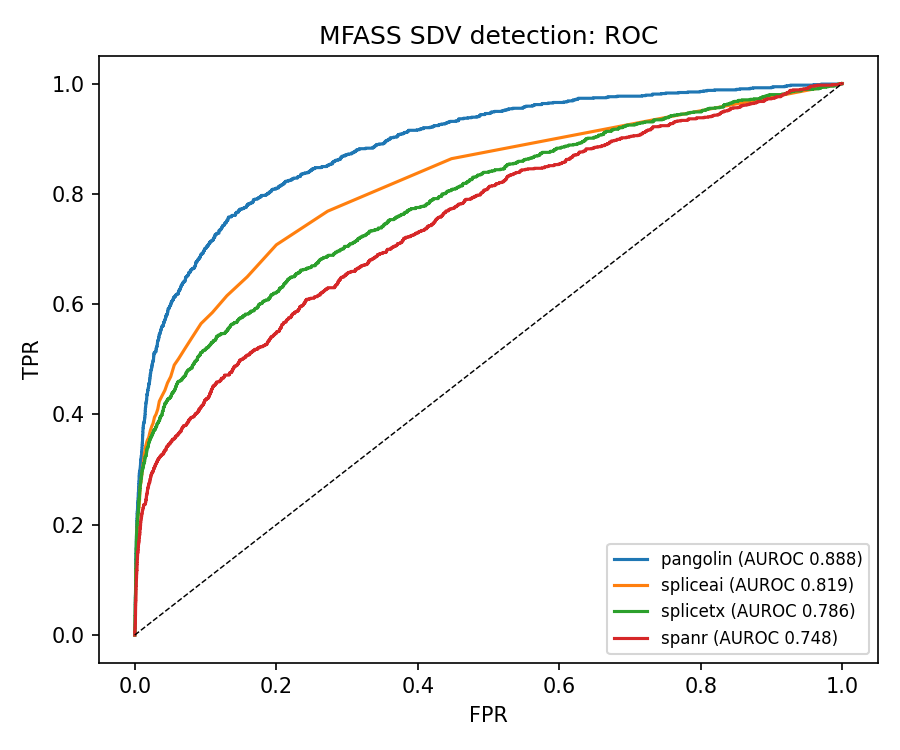
\includegraphics[width=0.70\textwidth]{../results/fig_roc.png}
\caption{ROC for splice-disrupting-variant detection. Pangolin shows the strongest
ROC performance; all modern tools exceed the legacy SPANR baseline.}
\end{figure}

\begin{figure}[h]
\centering
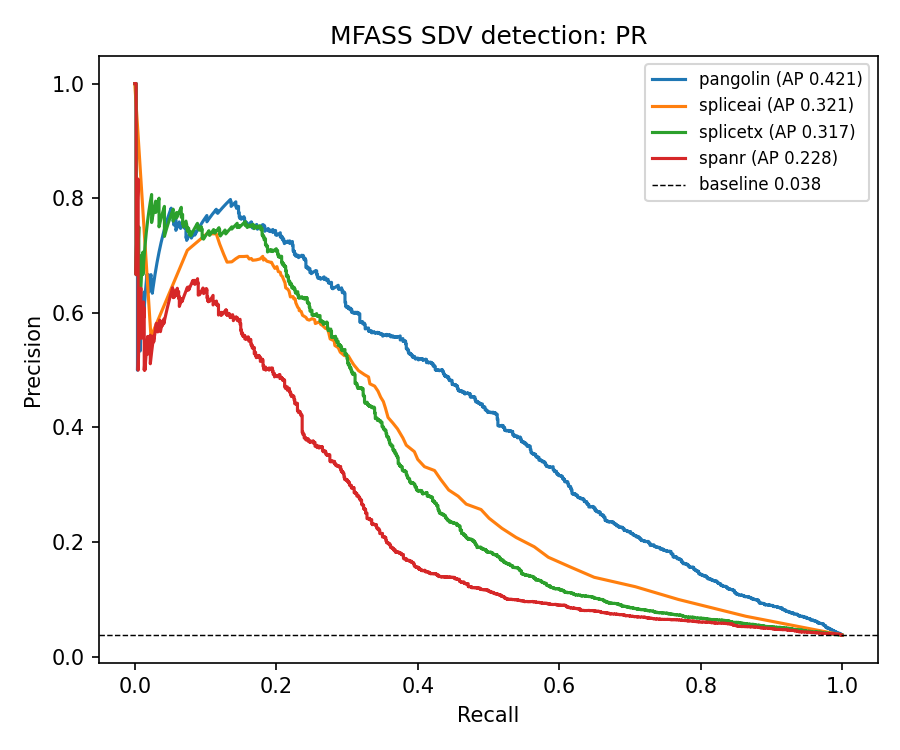
\includegraphics[width=0.70\textwidth]{../results/fig_pr.png}
\caption{Precision-recall for the same task (dashed line is the 0.038 positive
base rate). The ranking is consistent with the ROC view.}
\end{figure}

\textbf{Finding 1: Pangolin is the strongest predictor}, by a clear margin on both
AUROC and average precision, and its AP confidence interval does not overlap those
of the other tools. \textbf{Finding 2: all three modern predictors beat the legacy
SPANR model.} \textbf{Finding 3: the ranking reproduces the relative ordering the
Pangolin authors reported}, which is a correctness check on the scoring pipeline.

\textbf{Finding 4 (output granularity): in these outputs SpliceAI's scores are more
discretized than Pangolin's.} SpliceAI reports its delta to two decimals and assigns
exactly zero to most variants away from splice sites: 55\% of non-disrupting variants
but only 14\% of SDVs score zero, so the zeros are genuine no-effect calls (zeros are
depleted of SDVs, 0.96\% versus the 3.79\% base rate), not an artifact. Pangolin
instead uses a continuous range (about 1\% of variants near zero). This finer score
resolution may contribute to Pangolin's stronger ranking here.

\textbf{Finding 5 (consensus): combining does not help.} A logistic-regression
consensus of the three modern predictors, trained and evaluated on an
\emph{exon-grouped} 50/50 split (no exon appears in both train and test), reaches
held-out AP 0.443 versus Pangolin's 0.442 on the same split, a difference far
inside the bootstrap interval, and a slightly lower AUROC (0.890 versus 0.893). A
rank-average consensus is worse (AP 0.372). The fitted model essentially relies on
Pangolin alone (standardized coefficient 2.0, versus near zero or negative for the
others). For this MFASS benchmark, Pangolin is the strongest single predictor.

\section{Where the tools fail}
The aggregate ranking hides where the predictions break down. We stratified
splice-disrupting-variant recall by the distance of each variant to the nearest
splice site, computed from the MFASS minigene construct annotation and cross-checked
against an independent genomic-coordinate distance (Pearson $r=0.997$), comparing
all four tools at a common operating point: the score threshold that gives a 10\%
false-positive rate on non-disrupting variants.

\begin{figure}[h]
\centering
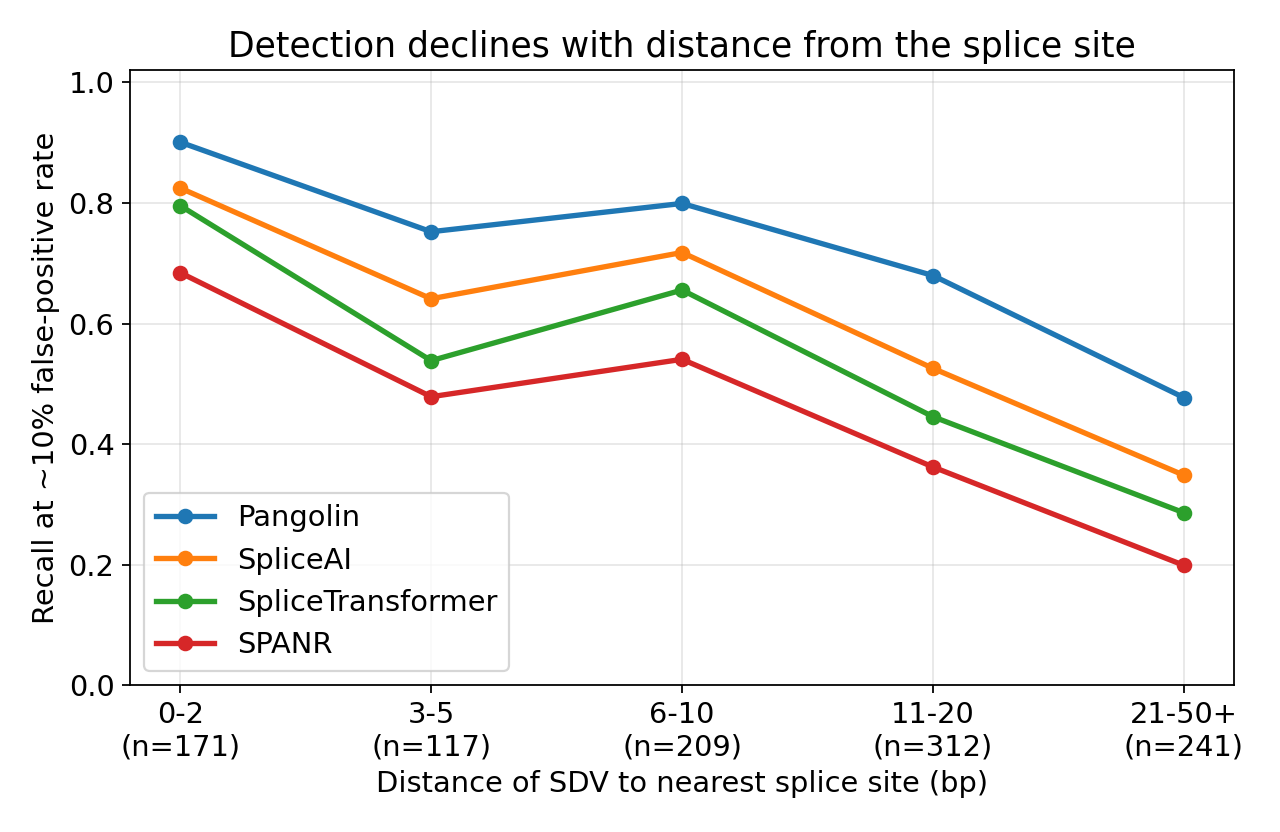
\includegraphics[width=0.78\textwidth]{../results/fig_failuremode.png}
\caption{Recall of splice-disrupting variants, at a common 10\% false-positive
rate, as a function of distance to the nearest splice site. Every tool detects
splice-site-proximal disruptions well and degrades with distance from the splice site.}
\end{figure}

Recall declines with distance from the splice site for every tool (Figure~3).
Within 2\,bp of a splice site the modern tools recover 80 to 90\% of disrupting
variants (Pangolin 0.90, SpliceAI 0.82, SpliceTransformer 0.80); beyond 20\,bp their
recall falls to 0.48, 0.35, and 0.29 respectively, and SPANR to 0.20. More than half
of the disrupting variants (53\%) lie more than 10\,bp from a splice site, and even
Pangolin, the best tool, detects only 59\% of them.

Most strikingly, 22\% of all disrupting variants (228 of 1{,}050) are missed by
every one of the four tools at this operating point. These shared misses sit
predominantly away from the splice site: 75\% lie more than 10\,bp from a splice
site, and 162 of 228 (71\%) are exonic. They are consistent with exon-interior
regulatory disruptions, including possible exonic splicing enhancer or silencer
effects, that splice-site models are not built to capture, the class of variant
MFASS was designed to expose. The practical implication is that these tools are
strongest for splice-site-proximal variants but require caution for exon-interior
variants, where roughly one in five disrupting variants is invisible to all current
predictors.

\section{What this shows, and what it does not}
It shows that, against a multiplexed experimental splicing assay, Pangolin detects
splice-disrupting variants better than SpliceAI, SpliceTransformer, and SPANR, that
all modern tools beat the legacy baseline, and that a simple consensus does not
improve on the best single tool. Several caveats bound the claim. First, the
predictors were trained on genomic and transcriptomic data and may have encountered
the wild-type splice sites of these exons during training, so this is a realistic
benchmark rather than a fully held-out one; this is standard for the field and
applies to all tools. Second, MFASS is an in-vitro minigene assay in a single
cellular context, so it does not capture tissue-specific or full-length-gene
effects, and we therefore used the tissue-aware tools in a tissue-agnostic setting.
Third, all predictors are scored as disruption magnitudes against a loss-of-function
label; a directional or tissue-resolved analysis is left for future work. The
contribution is a reproducible head-to-head benchmark, not a claim of clinical validation.

\section{Reproducibility and data processing}
The labels and continuous readout are the public MFASS measurements \cite{mfass};
all predictor scores are produced by the public models run through Proto
\cite{proto}. Variants whose reported alleles are on the minus strand were normalized to
the plus strand before scoring; for the three Proto-scored modern predictors, full
coverage of 28{,}972 of 28{,}972 variants confirms no variant was silently dropped,
and SPANR covers slightly fewer because MFASS provides precomputed SPANR scores for
only a subset. SpliceAI returns no score for variants outside an
annotated gene; these were assigned a delta of zero, a minority as shown by the
depletion of SDVs among zero-scored variants. Every number is reproduced by
\texttt{score\_one\_tool.py} (scoring on GPU) and \texttt{analyze.py} (metrics,
consensus, and figures) from the public dataset.

\section{Data and code availability}
All code, the per-tool variant scores, the benchmark and failure-mode outputs, and
the figures are openly available at \url{https://github.com/brhanufen/spliceconsensus}
and archived on Zenodo (doi:10.5281/zenodo.20948820). The benchmark and all figures reproduce on
a CPU in about a minute from the committed scores and a slim labels file, with no large
download. The MFASS dataset is from Chong et al. \cite{mfass}
(\url{https://github.com/KosuriLab/MFASS}); the predictors are the public SpliceAI
\cite{spliceai}, Pangolin \cite{pangolin}, SpliceTransformer \cite{splicetransformer},
and SPANR \cite{spanr} models, run through the Proto tool ecosystem \cite{proto}.

\section{Author contributions, competing interests, and funding}
B.F.Z. designed the benchmark, ran the analyses, generated the figures, and wrote the
manuscript. Z.A. contributed to the conceptual discussion and revised the manuscript.
Both authors read and approved the final manuscript. The authors declare no competing
interests. No specific funding was received for this work.

\begin{thebibliography}{9}
\bibitem{splicingdisease} Scotti, M.M. and Swanson, M.S. RNA mis-splicing in disease. \emph{Nature Reviews Genetics} 17, 2016. doi:10.1038/nrg.2015.3.
\bibitem{pangolin} Zeng, T. and Li, Y.I. Predicting RNA splicing from DNA sequence using Pangolin. \emph{Genome Biology}, 2022. doi:10.1186/s13059-022-02664-4.
\bibitem{spliceai} Jaganathan, K., Kyriazopoulou Panagiotopoulou, S., McRae, J.F., et al. Predicting splicing from primary sequence with deep learning (SpliceAI). \emph{Cell}, 2019. doi:10.1016/j.cell.2018.12.015.
\bibitem{splicetransformer} You, N., Liu, C., Gu, Y., et al. SpliceTransformer predicts tissue-specific splicing linked to human diseases. \emph{Nature Communications}, 2024. doi:10.1038/s41467-024-53088-6.
\bibitem{mfass} Chong, R., Insigne, K.D., Yao, D., Burghard, C.P., Wang, J., Hsiao, Y.-H.E., Jones, E.M., Goodman, D.B., Xiao, X., and Kosuri, S. A multiplexed assay for exon recognition reveals that an unappreciated fraction of rare genetic variants cause large-effect splicing disruptions. \emph{Molecular Cell} 73, 183-194.e8, 2019. doi:10.1016/j.molcel.2018.10.037.
\bibitem{spanr} Xiong, H.Y., Alipanahi, B., Lee, L.J., et al. The human splicing code reveals new insights into the genetic determinants of disease (SPANR). \emph{Science} 347, 2015. doi:10.1126/science.1254806.
\bibitem{proto} Merchant, A.T., Guo, D., Viggiano, B., et al. A high-level programming language for generative biology with Proto. \emph{bioRxiv} 2026.06.22.733870, 2026. doi:10.64898/2026.06.22.733870.
\end{thebibliography}
\end{document}
